%%%% Better Poster latex template example v1.0 (2019/04/04)
%%%% GNU General Public License v3.0
%%%% Rafael Bailo
%%%% https://github.com/rafaelbailo/betterposter-latex-template
%%%% 
%%%% Original design from Mike Morrison
%%%% https://twitter.com/mikemorrison

\documentclass[a0paper,fleqn]{betterposter}

%%%% Uncomment the following commands to customise the format

%% Setting the width of columns
% Left column
\setlength{\leftbarwidth}{0.25\paperwidth}
% Right column
\setlength{\rightbarwidth}{0.235\paperwidth}

%% Setting the column margins
% Horizontal margin
%\setlength{\columnmarginvertical}{0.05\paperheight}
% Vertical margin
%\setlength{\columnmarginhorizontal}{0.05\paperheight}
% Horizontal margin for the main column
\setlength{\maincolumnmarginvertical}{0.05\paperheight}
% Vertical margin for the main column
%\setlength{\maincolumnmarginhorizontal}{0.15\paperheight}

%% Changing font sizes
% Text font
%\renewcommand{\fontsizestandard}{\fontsize{28}{35} \selectfont}
% Main column font
%\renewcommand{\fontsizemain}{\fontsize{28}{35} \selectfont}
% Title font
%\renewcommand{\fontsizetitle}{\fontsize{28}{35} \selectfont}
% Author font
\renewcommand{\fontsizeauthor}{\fontsize{35}{20} \selectfont}
% Section font
%\renewcommand{\fontsizesection}{\fontsize{28}{35} \selectfont}

%% Changing font sizes for a specific text segment
% Place the text inside brackets:
% {\fontsize{28}{35} \selectfont Your text goes here}

%% Changing colours
% Background of side columns
%\renewcommand{\columnbackgroundcolor}{black}
% Font of side columns
%\renewcommand{\columnfontcolor}{gray}
% Background of main column
%\renewcommand{\maincolumnbackgroundcolor}{empirical}
%\renewcommand{\maincolumnbackgroundcolor}{theory}
%\renewcommand{\maincolumnbackgroundcolor}{methods}
%\renewcommand{\maincolumnbackgroundcolor}{intervention}
% Font of main column
%\renewcommand{\maincolumnfontcolor}{gray}

\begin{document}	
\betterposter{
%%%%%%%% MAIN COLUMN

\maincolumn{
%%%% Main space

\textbf{Where} did all this waste come from?
\\translated into \textbf{plain English}.
\\\textbf{Emphasize} the important words.
}{
%%%% Bottom space
%% This fills the space between the content and the logo
\vfill
%% Institution logo
\begin{flushright}

\includegraphics[height=0.1\textwidth]{img/logoUL_white}
\hspace{30pt}

\includegraphics[height=0.1\textwidth]{img/brightway}
\vspace{10pt}
\end{flushright}
}

}{
%%%%%%%% LEFT COLUMN

\title{WasteFootprint}
{\fontsizesection\selectfont\textbf{a flexible python tool for analysing\\ supply-chain waste flows in LCA}}\\

\vspace{10pt}
\author{Elizabeth Lanphere, Stewart Charles McDowall, Stefano Cucurachi, Carlos Filipe Blanco Rocha}
\vspace{30pt}
\institution{CML, Leiden University, The Netherlands}

\section{What?}
Here is an itemised list:
\begin{itemize}
\item The first item.
\item The second item.
\item The third item.
\end{itemize}

\section{Why?}
Here is a diagram:
% \begin{center}

% \end{center}

\section{How?}


\section{What next?}
This is a great poster format!

\vfill
\begin{center}

\includegraphics[width=0.4\textwidth]{img/qr_code}\\
{\fontsizesection\selectfont\textbf{Github repo}}
\end{center}

}{
%%%%%%%% RIGHT COLUMN
{\fontsizesection\selectfont\textbf{Step by step through the code}}\\

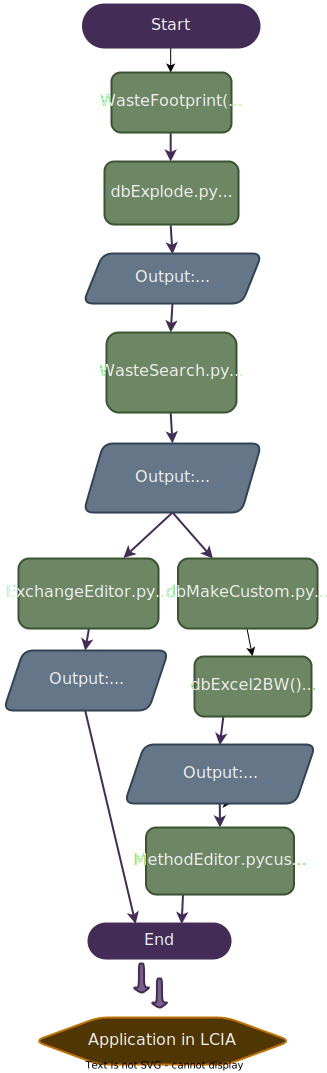
\includegraphics[width=\textwidth]{img/Flowchart_WasteFootprint}
}
\end{document}
